\documentclass[]{sigplan-proc}
\usepackage{graphicx}
\usepackage{epstopdf}
\usepackage{url}
\usepackage{listings}
\renewcommand{\topfraction}{0.85}
\renewcommand{\textfraction}{0.1}

\conferenceinfo{TBD}{TBD}
\CopyrightYear{2012}
\crdata{}

\begin{document}

\title{The Mysterious Case of Lustre Networking at 100 Gigabits}
\subtitle{A study of LNET behavior over high bandwidth, high latency networks}

\numberofauthors{6}
\author{
\alignauthor Scott Michael\\
	\affaddr{Indiana University}\\
	\affaddr{Bloomington, IN 47408}\\
	\email{scamicha@iu.edu}
\alignauthor Liang Zhen\\
        \affaddr{Whamcloud Inc.}\\
        \affaddr{Danville, CA 94526}\\
        \email{liang@whamcloud.com}
\alignauthor Robert Henschel\\
        \affaddr{Indiana University}\\
        \affaddr{Bloomington, IN 47408}\\
        \email{henschel@iu.edu}
\and
\alignauthor Stephen Simms\\
	\affaddr{Indiana University}\\
	\affaddr{Bloomington, IN 47408}\\
	\email{ssimms@indiana.edu}
\alignauthor Eric Barton\\
        \affaddr{Whamcloud Inc.}\\
        \affaddr{Danville, CA 94526}\\
        \email{eeb@whamcloud.com}
\alignauthor Matthew Link\\
	\affaddr{Indiana University}\\
	\affaddr{Bloomington, IN 47408}\\
	\email{mrlink@indiana.edu}		
}

\maketitle

\begin{abstract}

  As part of the SCinet Research Sandbox at the Supercomputing 2011 conference, Indiana University utilized a
  dedicated 100 Gbps wide area network (WAN) link spanning more than 3,500 km (2,175 mi) to demonstrate the
  capabilities of the Lustre high performance parallel file system in a high bandwidth, high latency WAN
  environment. This demonstration functioned as a proof of concept and provided an opportunity to study
  Lustre's performance over a 100 Gbps WAN. To characterize the performance of the network and file system a
  series of benchmarks and tests were undertaken. These included low level iperf network tests, Lustre
  networking (LNET) tests, file system tests with the IOR benchmark, and a suite of real-world applications reading
  and writing to the file system. All of the tests and benchmarks were run over a the WAN link with a latency
  of 50.5 ms. In this article we describe the configuration and constraints of the demonstration and focus in
  on the key findings and discoveries made regarding the Lustre networking layer for this extremely high
  bandwidth and high latency connection. Of particular interest is the relationship between the {\tt peer\_credits}
  and {\tt max\_rpcs\_in\_flight} settings when considering LNET performance.

\end{abstract}

\category{H.3.4}{Information Storage and Retrieval}{Systems and Software}[Distributed systems, Performance evaluation (efficiency and effectiveness)]
\category{C.2.2}{Computer-\linebreak Communication Networks}{Network Protocols}[Protocol architecture (OSI model),
Routing protocols]

\terms{Algorithms, Performance}

\keywords{WAN file systems, Lustre, Data Superconductor}
\vspace{0.25in}
\section{Introduction}\label{sec:intro}

The SCinet Research Sandbox (SRS) at the Supercomputing 2011 (SC11) conference encourages institutions to
showcase new and innovative technologies in the area of networking. For the demonstration SCinet, in
collaboration with ESnet and Internet2, provided all SRS participants with a 100 Gbps network connection from
the SC11 show floor to the Internet2 backbone. This link provided an end-to-end connection from the IU booth
on the SC11 show floor to the IU Data Center in Indianapolis, Indiana. 

The overall goal of the IU entry into the SRS was to demonstrate the use of a Lustre file system in scientific
applications over the 100 Gbps wide area network (WAN) spanning from Seattle, Washington to Indianapolis,
Indiana, a distance in excess of 3,500 km (2,175 mi). A diagram of the network and routing points is given in
figure \ref{fig:network}. Such a use case is of obvious intrest for geographically distributed workflows; for
example, when data sources, such as remote sensors are in locations very distant from computational resources
used to analyze the data. Though the overall demonstration was ultimately successful, IU achieved the highest
reported throughput (6.2 GB/s) with scientific applications running across the WAN, the focus of this article
is the performance of and lessons learned about the Lustre networking layer, LNET.

\begin{figure*}[t]
\begin{center}
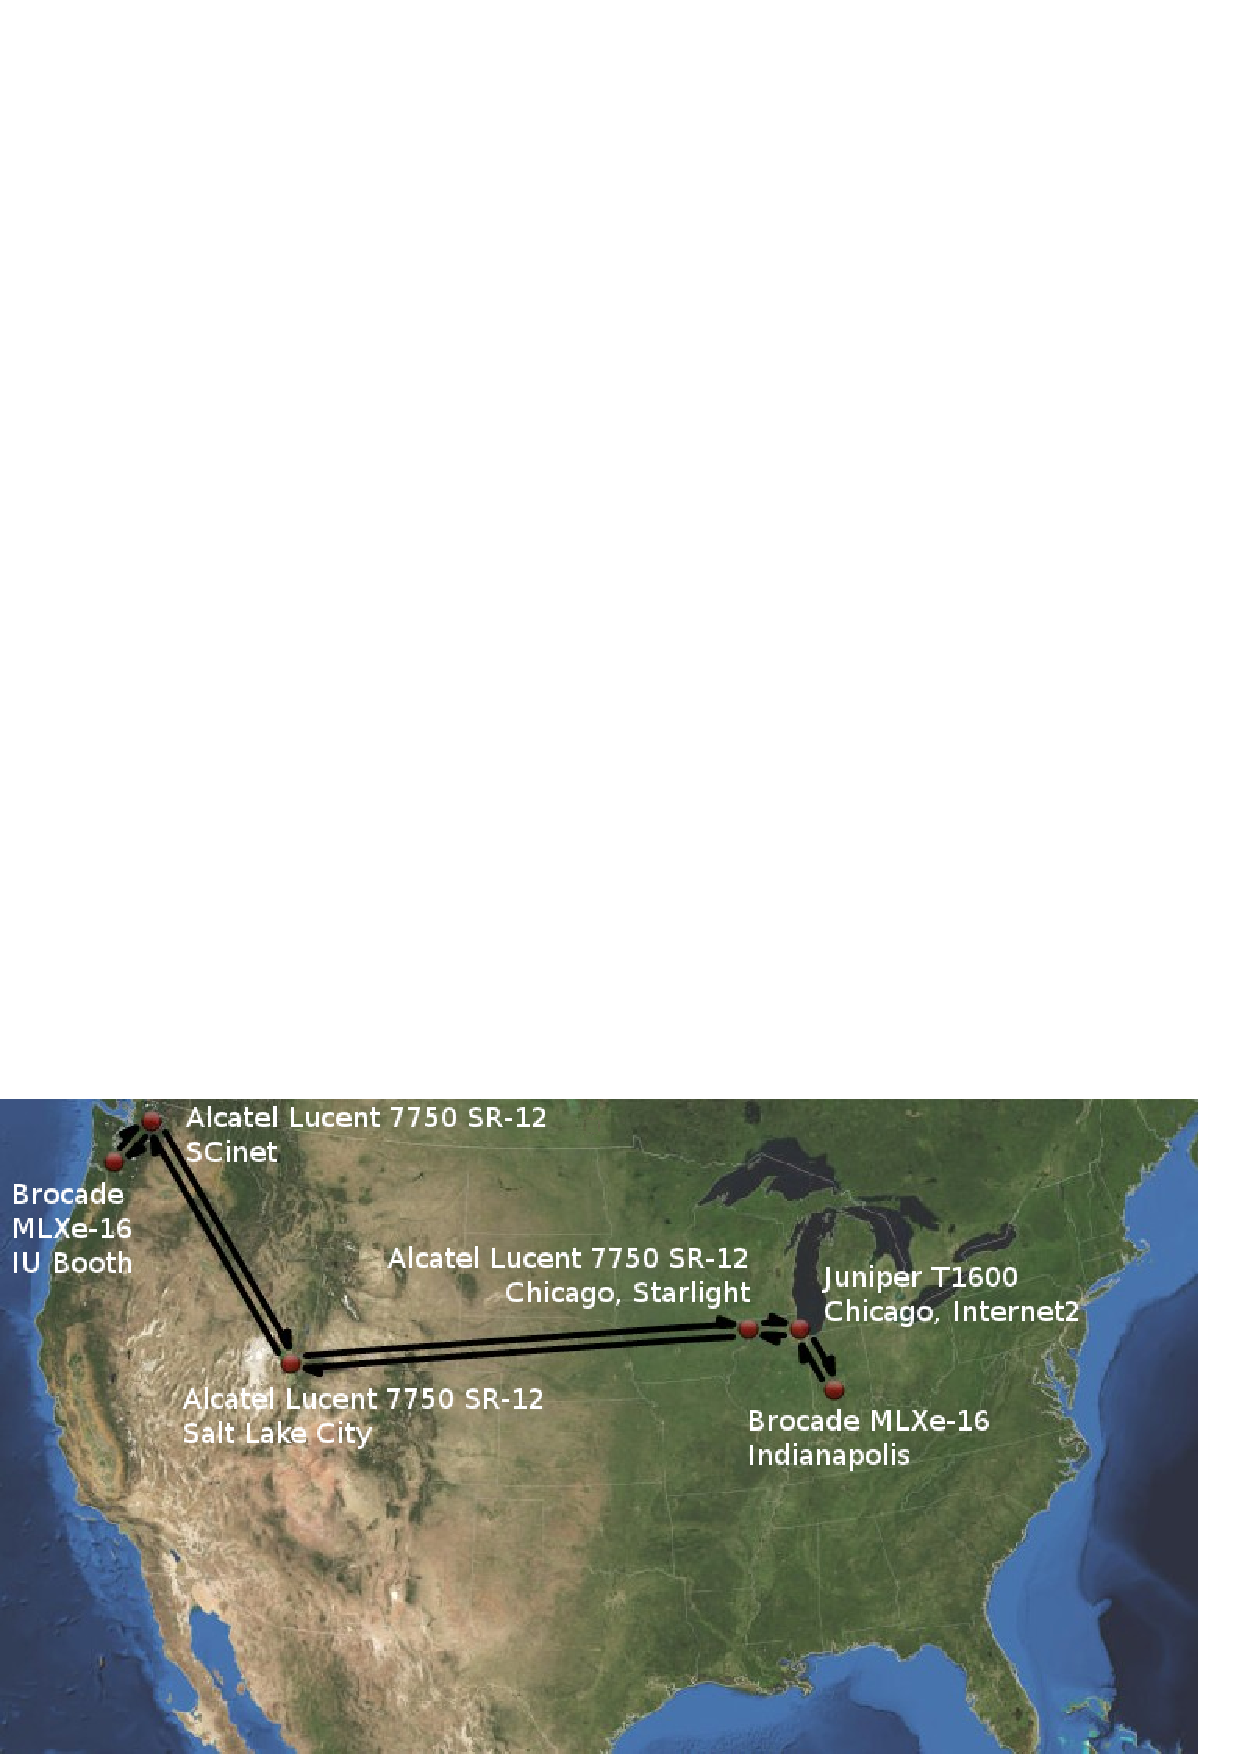
\includegraphics[width=0.80\textwidth]{figures/network.png}
\caption{Hardware setup}
\label{fig:hardwaresetup}
\end{center}
\end{figure*}

Access to the 100 Gbps WAN was facilitated and coordinated by SCinet. Each participant was given time slots
for exclusive use of the network. The slots were evenly distributed from Saturday, November 12th to Thursday,
November 17th. In total, IU was provided nine test slots for a combined 16 hours. All testing that required
access to the network links had to be performed during those times, from setting up the actual end to end
network connectivity to performing file system and application tests. In addition, we were provided five
demonstration slots for a total of four hours. Those time slots were used to showcase the capabilities of the
system in the IU booth. All results described in this article were obtained in the 20 hours of demonstration
and test time.

The fact that this study was performed in such a limited timeframe influenced the measurements we were able to
take. In addition to the fact that the time allotted to IU was fairly short, the initial connection of the 100
Gbps link required some fine tuning of the routing elements between Seattle and Indianapolis to achieve an
eventual peak throughput of 96 Gbps on the TCP layer \cite{henschel2012}. Although the network issues were
eventually resolved, this phase of the troubleshooting consumed nearly half of the time allocated to IU,
leaving approximately 10 hours for troubleshooting and gathering data on LNET, file system benchmarks, and the
performance of  scientific applications.

This paper is structured as follows: Section \ref{sec:LNET} gives a brief technical overview of the LNET layer
of Lustre with particular attention paid to remote procedure calls (RPCs) and peer credits. Section
\ref{sec:usecase} describes in detail the SRS use case, including the hardware setup that was used for the SRS
demonstration and the particulars of the Lustre installation and software tools used. Section
\ref{sec:results} describes the results obtained from measurements of the Lustre networking layer. In section
\ref{sec:discussion} we offer some hypotheses explaining the results and compare to previous work. A summary and conclusion follows in section \ref{sec:conclusion}.

\section{The Lustre Networking Protocol}\label{sec:LNET}

\subsection{Lustre Remote Procedure Calls}

\subsection{Lustre Peer Credits}
 

\section {The SC11 Example Case}\label{sec:usecase}

\subsection{Hardware}\label{sec:hardware}

Figure \ref{fig:hardwaresetup} shows the final configuration that was used between Seattle and
Indianapolis. IBM provided 31 servers that functioned as compute nodes as well as the 16 storage servers that
were attached to the DataDirect Networks (DDN) storage devices. Brocade and Ciena provided the routing
equipment that enabled the network link from the show floor to Indianapolis.

The configurations of the compute cluster, storage, and networking components were identical in both Indianapolis and
Seattle. The core networking component at each endpoint was a Brocade MLXe-16 router that provided a 100 Gbps
Ethernet connection to the Ciena optical terminal managed by Internet2. The core router also provided a 10
Gbps link to an IBM BNT G8264 OpenFlow enabled switch at each endpoint. These switches were connected at 10 Gbps
over a separate Internet2 connection. The 31 compute servers and 16 Lustre storage
servers were attached directly to the Brocade core router at 10 Gbps using Twinax cables and Brocade 1860
dual-port adapters.

The compute servers were IBM System x iDataPlex dx360 M3 systems, each configured with dual Intel Xeon E5645
6-core 2.40 GHz processors, 24 GB of DDR3 RAM, a Brocade 1860 adapter, and a 250 GB SATA hard drive. The
object storage servers (OSS) were IBM System x iDataPlex dx360 M3 servers each configured with an Intel Xeon
E5645 6-core 2.40 GHz processor, 48 GB of DDR3 RAM, a Brocade 1860 adapter, and a 1 TB SATA hard drive. The
OSS nodes at each site were connected directly to a DDN SFA10000 via 8 Gb Fibre Channel (FC). The SFA10000
drove five 60-slot storage enclosures configured with 2 TB SATA disk drives. The metadata server was identical
to the compute servers, except it had 96 GB of RAM and was directly connected to a DDN EF3015 RAID system that
contained twelve 300 GB 15K RPM SAS disk drives for Lustre metadata.

Due to space constraints on the show floor server density was important. The dual-port Brocade 1860 adapters
were able to saturate the 8 Gb FC links as well as the 10 Gbps Ethernet links simultaneously, allowing the use
of rack dense IBM iDataPlex servers with only one PCI-Express slot available. The throughput of the DDN
SFA10000 allowed us to use a single storage system for the Lustre OSS nodes at each site.

\begin{figure*}[t]
\begin{center}
\includegraphics[width=0.80\textwidth]{figures/hardware.png}
\caption{Shown here is the hardware configuration used for the SRS demonstration. An IBM iDataPlex cluster and
  Lustre file system were connected to a Brocade 100 Gpbs MLXe-16 router at each endpoint. The IBM routing
  equipment connected to the Brocade routers was used for the OpenFlow component of the demonstration and is
  not discussed in this article. }
\label{fig:hardwaresetup}
\end{center}
\end{figure*}

\subsection{Network}

Before shipping equipment to the show floor in Seattle to participate in the SRS, the demonstration
configuration was assembled in the IU machine room for testing.  There we performed tests with the two Brocade
MLXe routers connected back to back with the 100 Gbps connection spanning a few meters.  Local network tests
across this connection showed a latency of 0.24 ms and maximum stable performance of 98 Gbit/sec using TCP
iperf \cite{iperf2012}.

The network link that was used for this demonstration provided end to end 100 Gbps connectivity from the IU
booth on the SC11 show floor in Seattle to the IU Data Center in Indianapolis. Indiana University worked with
Internet2 to upgrade the existing link from Chicago to Indianapolis to 100 Gbps. Internet2 and ESnet provided access to the 100 Gbps link from Chicago to Salt Lake City and on to
Seattle. In Seattle and on the show floor, SCinet was responsible for the network link. The connection from
Salt Lake City to Seattle had been established at 100 Gbps only two weeks prior to SC11.

Once the link was established, we measured a latency of 50.5 ms between the compute cluster in Seattle and the
storage cluster in Indianapolis. Initial TCP iperf tests had shown good performance for two
parallel streams, each at 10 Gbps. However, when adding more iperf streams to the link, performance dropped
and throughput become unstable. We tuned two specific parts of the network to arrive at a stable 80 Gbps
throughput with TCP iperf. Our initial hardware setup included a Brocade VDX switch between the compute and
storage nodes and the Brocade MLXe router. The VDX was used to aggregate the 47 server links into 12 that were then
routed by the MLXe into the Ciena optical terminal. Despite our best efforts and assistance from Brocade
engineers we were unable to completely eliminate the performance impact of the VDX's link
aggregation. Directly connecting all compute and storage resources into the MLXe router eliminated the layer
of link aggregation that had been present on both sides of the connection. In addition, we worked with ESnet
to optimize the configuration of the three Alcatel-Lucent 7750 SR-12 routers in the path from Seattle to
Chicago. Those routers partition the 100 Gbps network traffic onto two 50 Gbps connections. Since our
end-to-end connection was mapped using two VLANs, we changed the configuration of those switches to statically
map one VLAN per 50 Gbps connection. Each VLAN contained half of the cluster nodes. Similar tuning was
performed for the connection from Chicago to Indianapolis, involving a Juniper T1600 and a Brocade MLXe
router. Following all of those modifications, we were able to put a stable 80 Gbps of TCP iperf traffic on the link, 40
Gbps per 50 Gbps connection and VLAN. This was achieved using eight servers on both sides of the link, four
per VLAN. Adding another single 10 Gbps stream to either of the connections resulted in congestion and
degraded performance. We then discovered that the two 50 Gbps connections were rated at slightly
less than 50 Gbps, which explained the congestion when adding the fifth server. However, when oversubscribing
the link by using all 30 compute nodes on each end, we were able to achieve a peak throughput of 96
Gbps. Those tuning steps yielded a stable connection only in one direction, from Seattle to Indianapolis. We
were never able to achieve similar results in the other direction. Due to time constraints, we focused our
efforts on just one direction.

\lstset{language=Bash, caption=Tuning parameters for the network, label=TuningListing}
\begin{lstlisting}
net.ipv4.tcp_rmem=4096 65536 167772160
net.ipv4.tcp_wmem=4096 65536 167772160
net.core.rmem_max=167772160
net.core.wmem_max=167772160
net.core.netdev_max_backlog=30000
eth2 txqueuelen 10000
eth2 mtu 9000
FlowControl off 
\end{lstlisting}

Listing \ref{TuningListing} shows the tuning parameters that were set on all nodes. We increased the maximum TCP buffer to 167 MB and increased the sending and receiving queues to 10000 and 30000. In addtion, we enabled MTU 9000 and configured all nodes to use the \texttt{tcp\_bic} network stack. Flow control was disabled on the network adapters and the routers.

\subsection{Software Configuration}




\section{Results}\label{sec:results}

\begin{figure}
\centering
\includegraphics[width=0.50\textwidth]{figures/default_pc_plot.eps}
\caption{}
\label{}
\end{figure}

\begin{figure}
\centering
\includegraphics[width=0.50\textwidth]{figures/32pc_plot.eps}
\caption{}
\label{}
\end{figure}

\begin{figure}
\centering
\includegraphics[width=0.50\textwidth]{figures/64pc_plot.eps}
\caption{}
\label{}
\end{figure}

\begin{figure}
\centering
\includegraphics[width=0.50\textwidth]{figures/all_pc_plot.eps}
\caption{}
\label{}
\end{figure}

\section{Discussion}\label{sec:discussion} 

\section{Conclusions}\label{sec:conclusions}
  
\section{Acknowledgements}

The authors would like to thank the contributions of our collaborators and technical staff. The following
staff at IU provided excellent support in the administration of the systems, testing applications,
visualization, technical writing, and project management: Edward Balas, Janae Cummings, Kurt Seiffert, Daphne
Siefert-Herron, Bill Sherman, Martin Swany, Jenett Tillotson, George Turner, Matt Allen, Nathan Heald and Josh Walgenbach. Internet2 provided network setup and support: Andrew Lee, Chris Robb, and Matthew Zekauskas. ESnet staff also provided setup and troubleshooting assistance: Evangelos Chaniotakis and Patrick Dorn.

The following vendors provided loaner hardware to support this project: Brocade loaned all the server host
adapters, two MLXe-16 100 Gbps switches, required Fibre Channel and Ethernet optics, and all the Twinax cables
used to connect the servers to the network. Ciena loaned optical equipment to Internet2 to enable the 100 Gbps
network from Chicago to Seattle. DataDirect Networks loaned two SFA10000 storage systems for Lustre object
storage targets and two EF3015 RAID arrays for Lustre metadata storage. IBM contributed 22 iDataPlex dx360 M3
servers for the project as well as two OpenFlow enabled BNT G8264 switches with required optics. Internet2
provided networking equipment to extend their 100 Gbps network from Chicago to Indianapolis.


\bibliographystyle{abbrv}
\bibliography{LNET}
\end{document}
